% xenon1t, v1.1

\chapter{The XENON1T Experiment}\label{ch:xe1t}

\paragraph{Abstract} This chapter provides an overview of the design and operation of the XENON1T detector and its associated subsystems. This is not an exhaustive treatment, instead focusing more on the wider picture than the equipment specifics, and the interested reader is recommended to Ref.~\cite{Aprile:2017aty} for a more complete description.

The XENON collaboration runs the world's leading WIMP direct detection experiment, and XENON1T is the third iteration in a series of ever-larger detectors~\cite{Angle:2007uj,Aprile:2011dd}. Built in central Italy at Laboratori Nazionali del Gran Sasso (LNGS), XENON1T is the largest and most sensitive xenon dual-phase time projection chamber (TPC) in the world at the time of commisioning, containing over $3200\1{kg}$ of xenon and a fiducial mass exceeding $1000\1{kg}$~\cite{Aprile:2017iyp}.

\section{Operational Overview}

The operation of the dual-phase TPC, such as the one employed by XENON1T, is as follows. When something interacts with a xenon atom inside the detector, it will produce excited atoms and liberated electrons. The excited atoms deexcite almost immediately, releasing photons that are collected by arrays of Hamamatsu R11410-21 photomultipler tubes (PMTs)~\cite{Aprile:2015lha} above and below the target. These photons provide what is called the \textit{S1} or \textit{prompt} signal. An external electric field drifts the electrons towards the liquid surface, where a second, much stronger field accelerates the electrons into the gas. These energetic electrons interact with the gas, creating more light that is again collected by the PMT arrays. This signal is variably called the \textit{S2}, \textit{delayed}, or \textit{ionization} signal. The time difference between the S1 and S2 is the amount of time the electrons were drifing, and yields the depth or $z$ coordinate of the interaction. The hit pattern on the top PMT array yields the $(x,y)$ position of the event, as the PMTs directly above the S2 location will see more photons and produce a stronger signal. Figure~\ref{fig:idealized_event} shows schematically a typical event.

\begin{figure}[htb]
\centering
	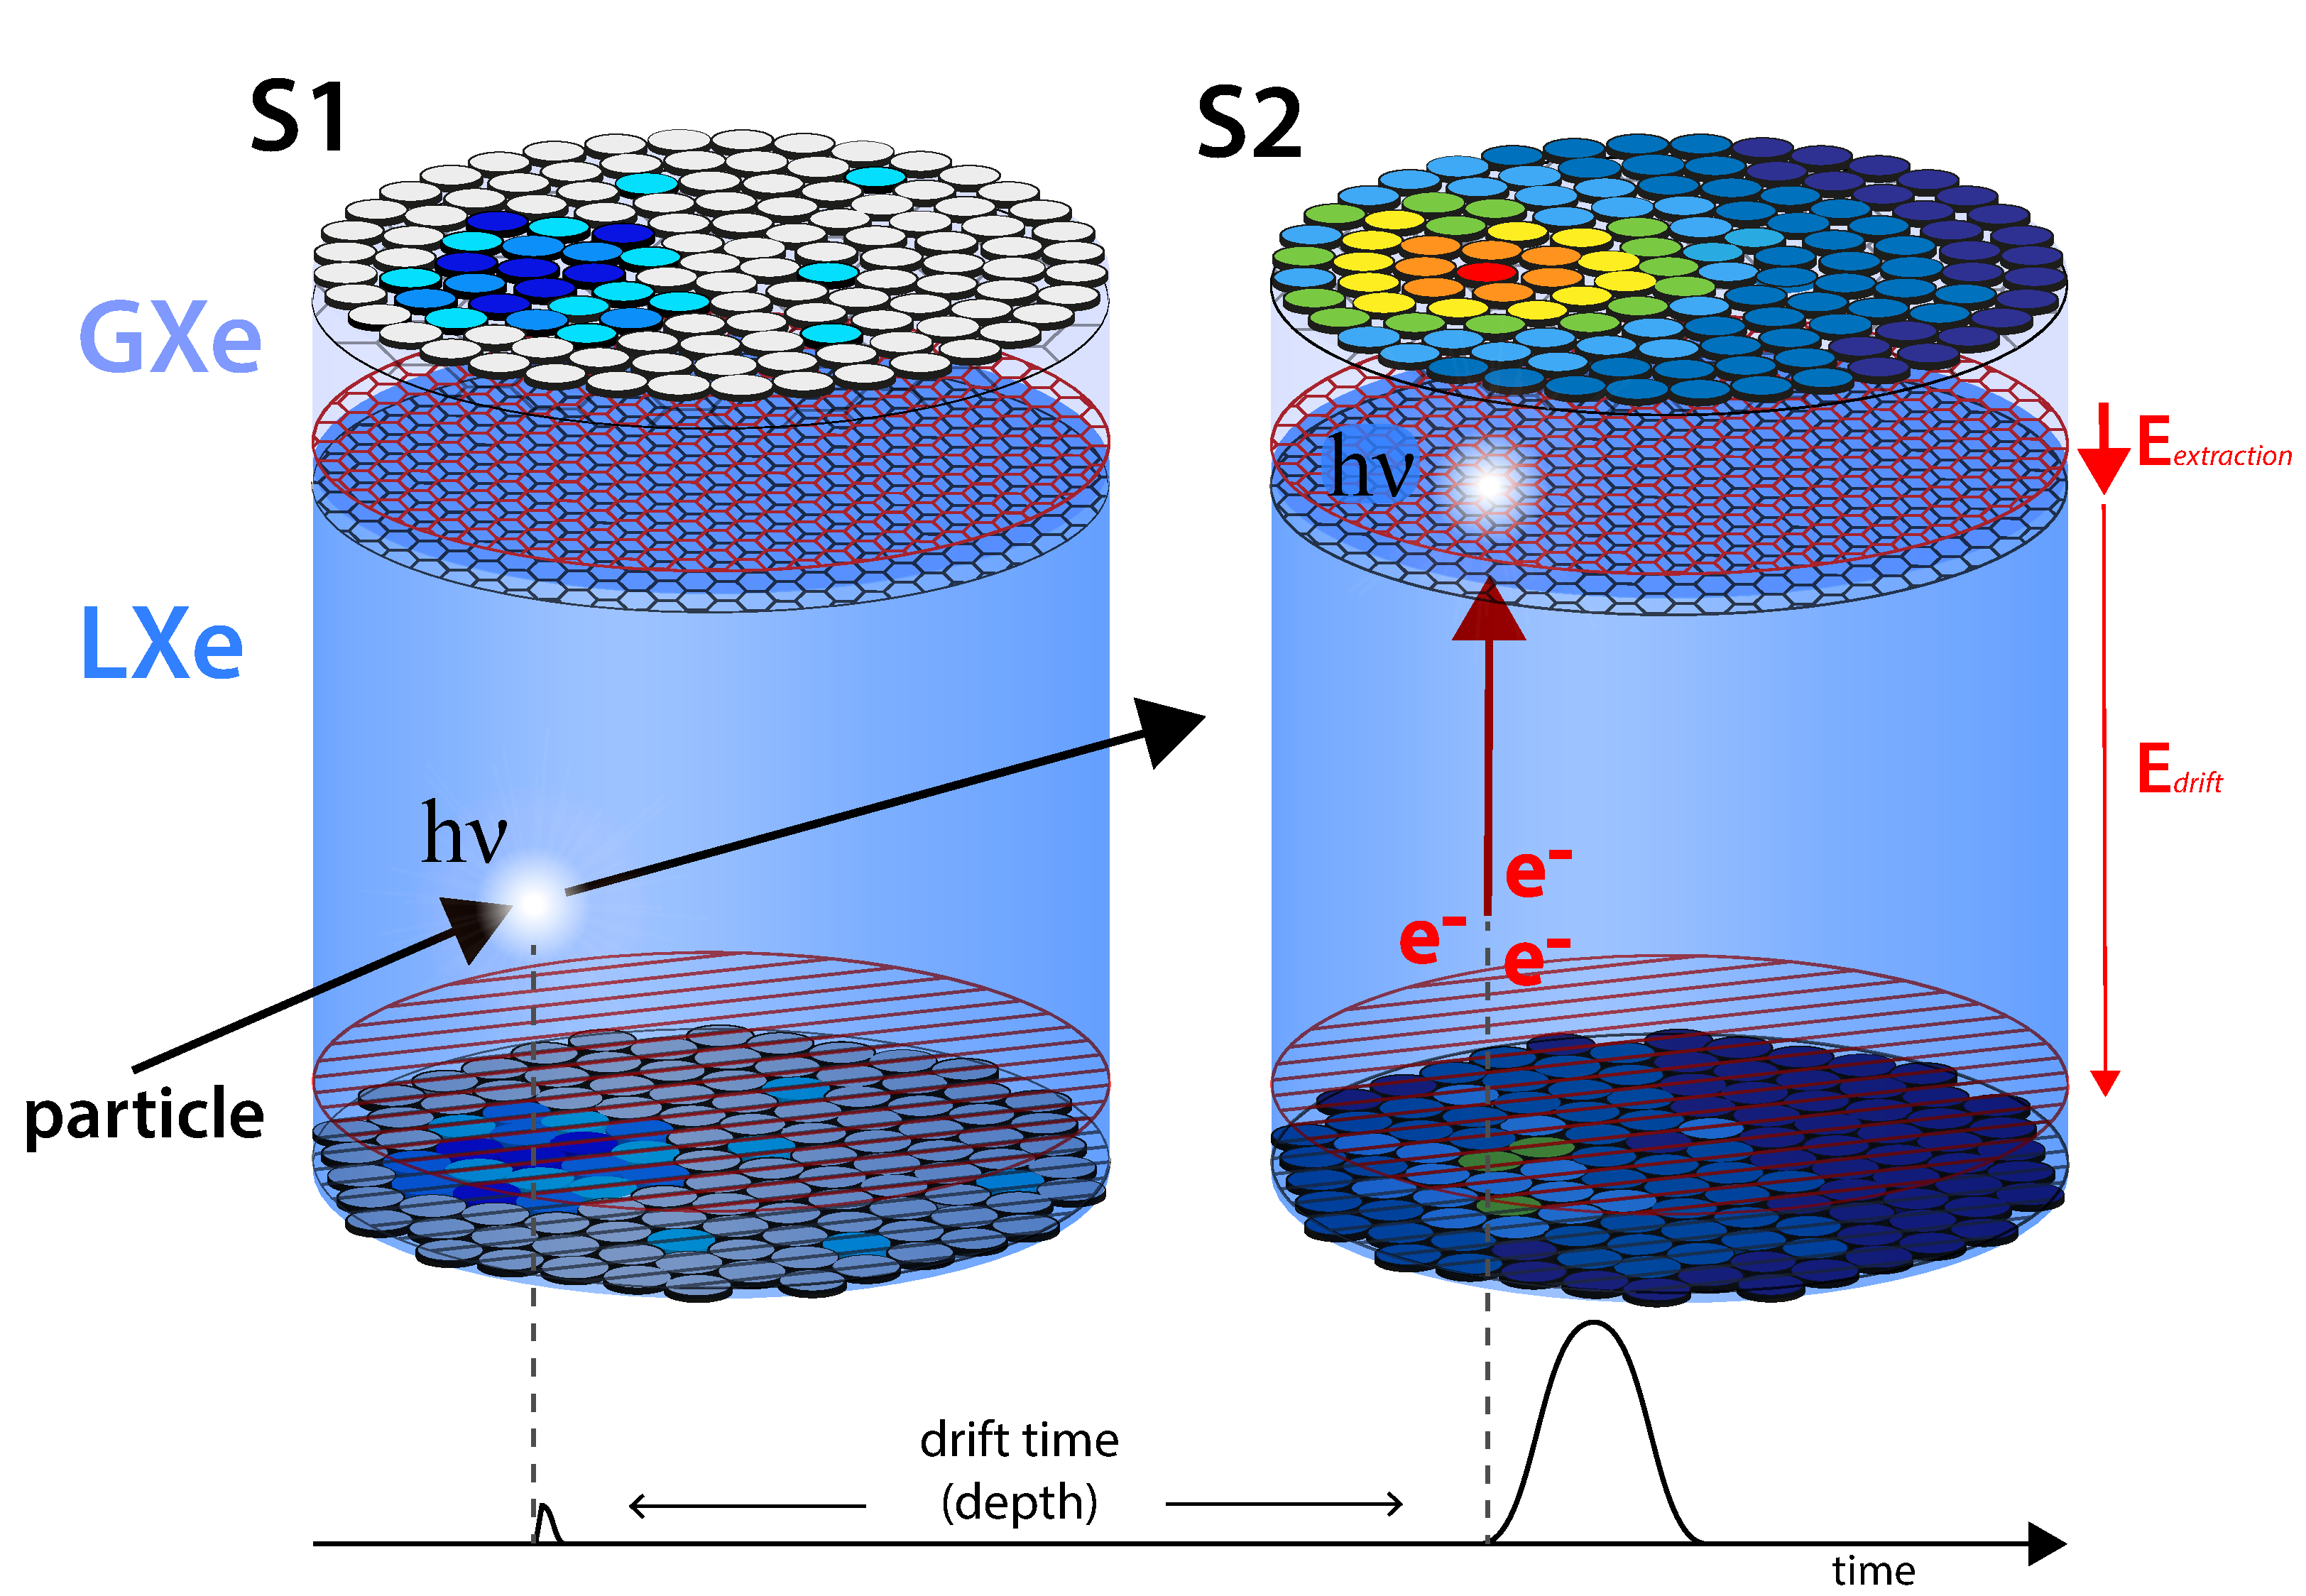
\includegraphics[width=0.8\textwidth]{figures/xe1t/tpc_xe1t_workingprinciple_v2.png}
	\caption{An idealized event inside a dual-phase TPC. An interaction in the liquid produces both prompt scintillation (\textit{S1}) and quasi-free electrons. Under the influence of an applied electric field, these electrons drift toward the liquid surface, where a second, stronger electric field extracts the electrons into the gas. These cause energetic collisions with the gasseous atoms, resuling in delayed scintillation (\textit{S2}). The time difference between signals indicates the depth of the interaction, while the hit pattern on the top PMTs indicates the transverse location.}\label{fig:idealized_event}
\end{figure}

The ability to reconstruct the position of an interaction in three dimensions yields the powerful ability of fiducialization. Additionally, xenon is very optically dense to high-energy photons. Because a significant source of background originates from materials surrounding the xenon, the combination of this self-shielding and the ability to determine where interactions occur allow us to define a fiducial volume where backgrounds are minimized.

\section{System Overview}

The XENON1T detector is composed of numerous subsystems to perform xenon handling, calibration, shielding, and data aquisition, and will be discussed here in some detail.

\subsection{Water tank}

The detector is housed in the center of a large tank of high-purity water, $10\1{m}$ in diameter and $10\1{m}$ in height. The rock overburden at LNGS reduces the cosmogenic muon flux to about 1 per square meter per hour~\cite{Bellini:2012te}, so muons will still regularly traverse the detector volume. However, by surrounding the detector with water, the Cherenkov radiation produced when muons (or particles from the showers they create) traverse this can be detected by an array of PMTs, and any coincident event in the TPC can be tagged~\cite{Aprile:2014zvw}.

Furthermore, the water also acts to shield the TPC from radioactivity in the surrounding rock. The trigger rate in the detector decreases significantly as the tank is filled, as shown in Figure~\ref{fig:waterlevel}.

\begin{figure}[htb]
    \begin{center}
    \includegraphics[width=0.8\textwidth]{figures/xe1t/water_level_part_2}
    \end{center}
    \caption{The trigger rate in XENON1T during the filling of the water tank. Surrounding the detector with several meters of water provides a reduction in trigger rate by two orders of magnitude.}\label{fig:waterlevel}.
\end{figure}

In the center of the tank stands the support structure that holds the cryostat, as well as the temporary platform which can be erected for maintenance on the TPC, cryostat, or surrounding systems.

\subsection{External calibration systems}

XENON1T has two primary external calibration systems. The first is known as the belt systems, and provide the ability to position radioactive sources at various locations surrounding the cryostat. The second is the deuterium-deuterium plasma fusion neutron generator~\cite{Lang:2017ymt} (see also Chapter~\ref{ch:ng}).

\subsubsection{Belt systems}

Three systems of belts are mounted in the water tank. Two of these systems have purely vertical travel (I-belts), and the third is capable of moving a source all the way underneath the detector along a secant (U-belt). These are located as shown in Figure~\ref{fig:belts}. Tungsten collimators mounted to carts on each belt allow $\gamma$s to be emitted in cones that illuminate much of the active volume.

\begin{figure}[htb]
\centering
    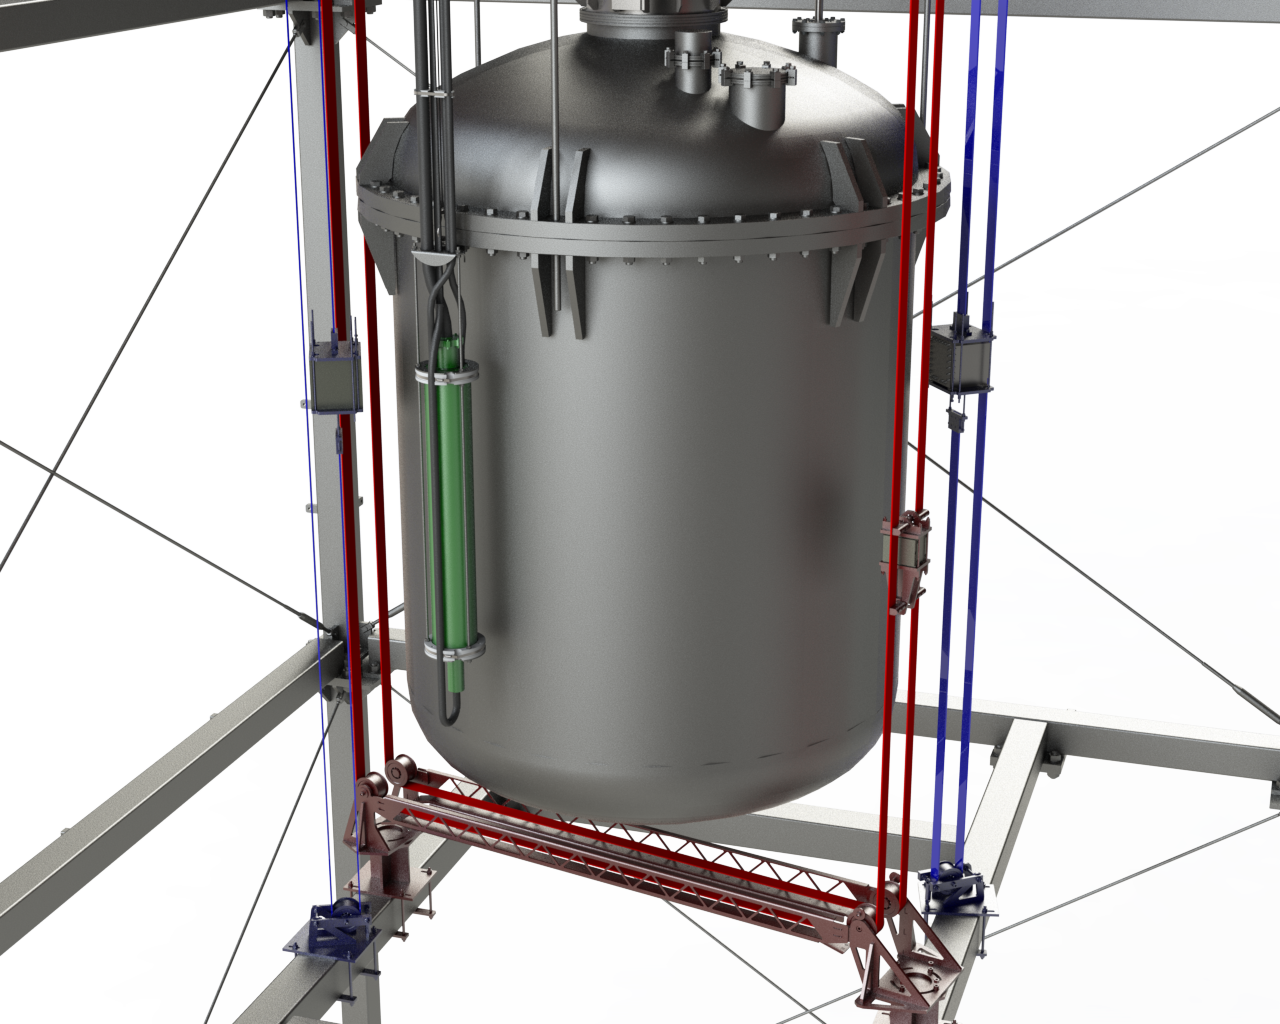
\includegraphics[width=0.8\textwidth]{figures/xe1t/cryo_belts_ng_colored}
    \caption{Placement of external calibration systems around the XENON1T cryostat. The neutron generator (green) is used for nuclear recoil calibrations, while the I-belts (blue) and U-belt (red) allow for the positioning of $\gamma$ sources to measure (among other things) self-shielding and electrical field distortion. The neutron generator can also be placed in two other locations around the cryostat (not shown) to provide a more uniform calibration.}\label{fig:belts}
\end{figure}

Sources of $^{137}$Cs, $^{228}$Th, and $^{241}$AmBe have been successfully deployed in these systems. A lead slug was mounted with the $^{241}$AmBe source to reduce the flux of high-energy $\gamma$s.

\subsubsection{Neutron generator}

While the increased size of XENON1T poses new challenges for calibration, it also offers new opportunities. The detector diameter is much larger than the mean free path of fast neutrons, so accurate reconstruction of multiple interaction vertices is possible. The energy deposited in an elastic interaction with a xenon nucleus is given by equation~\eqref{eq:doublescatter}.

\begin{equation}
\frac{E_{Xe}}{E_n} = \frac{2\frac{m_{Xe}}{m_n}(1-\cos\theta)}{\left(1+\frac{m_{Xe}}{m_n}\right)^2}
\label{eq:doublescatter}
\end{equation}

If the incident neutron energy $E_n$ is known, the deposited energy $E_{Xe}$ can be accurately measured. The masses of xenon and the neutron are $m_{Xe}$ and $m_n$, respectively, and $\theta$ is the scattering angle. By placing the neutron generator in a well-defined position next to the cryostat, the location of the neutron source is then known and accurate reconstruction of the scattering angle is possible.

A fast neutron travels at approximately $0.05\1{c}$, so will cross the detector in about $70\1{ns}$. While the temporal resolution is insufficient to resolve multiple S1s that occur in this time, the following S2 signals can be separated by tens or hundreds of microseconds. This is sufficient to perform accurate \textit{in situ} charge yield measurements, as demonstrated by LUX~\cite{Akerib:2016mzi}.

\subsection{Gas recirculation, purification, and cryogenics}

A large series of tubes and pipes exists to support the operation of the detector. This system is responsible for filling and emptying the detector, introducing radioactive sources into the detector for various calibrations, and maintaining the purity of the xenon in the detector by recirculating through hot zirconium getters. Two separate parallel lines, each containing pumps and a getter, provide increased xenon throughput as well as some redundancy in the event of maintenance requirements. A source box containing various internal calibration sources (including $^{83m}$Kr~\cite{Kastens:2010,Akerib:2017eql}, $^{220}$Rn~\cite{Aprile:2016pmc,Lang:2016zde}, and $\n{CH}_3\n{T}$~\cite{Akerib:2015wdi}) is connected to the gas system and allows the injection of sources both before and after the getters.

The paradigm for cooling is the same ``remote cooling'' configuration as was used in XENON100~\cite{Aprile:2011dd}. In this setup, cooling is provided by pulse tube refrigerators (PTRs) installed some distance from the TPC itself. Xenon gas from around the TPC diffuses upwards to the coldfingers, and the liquid xenon that condenses onto the colfingers flows back down pipes towards the TPC. This allows for easy maintenance of the cooling systems with only marginal impact on the system operation. Two redunandant PTRs, each rated for $250\1{W}$ of cooling at $177\1{K}$, are more than sufficient to provide the $\approx 150\1{W}$ of cooling necessary for stable operation. In the event of power loss or some other thermodynamic anomaly (for instance, failure of the insulation vacuum), backup liquid nitrogen cooling can maintain the system pressure at safe levels.

While electronegative impurities that emanate from materials are efficiently removed by the getters, noble element contaminants, such as krypton or argon, are not. One of these is the $\beta^-$ emitter $^{85}$Kr. Decays of this isotope contribute to the low-energy electronic recoil background and can be removed by cryogenic distillation, exploiting the different vapor pressures of xenon and krypton. A distillation column was constructed for this purpose, and successfully reduced the krypton level to the required $<0.2\1{ppt}$~\cite{Aprile:2015uzo,Aprile:2016xhi}. As krypton and argon are not produced in appreciable quantities once the xenon is safely underground, this purification only needs to be performed once. Additionally, the column can also be run in reverse mode to remove radon rather than krypton.

\subsection{Electronics and DAQ}

A variety of eletronics are housed in the service building adjacent to the water tank for the purpose of running the data acquisition (DAQ) systems. Each PMT requires connections for both signal and high voltage. PMT signals are fed through Phillips Scientific 776 amplifiers (providing a gain of 10) into CAEN V1724 ADC modules ($2.25\1{V}$ dynamic range, 14 bit resolution, $100\1{MHz}$ sample frequency) to digitize the traces. These are fed into a MongoDB noSQL database that acts as a circular buffer. Additionally, the waveforms for the top and bottom PMT arrays are summed and used to provide a high-energy veto. All signals with amplitude above $\sim 0.3\1{pe}$ are read asynchronously, zero-suppressed, and fed into the buffer database. Operating on this database is a program called the Event Builder, which monitors the data stream and saves any event-like patterns to disk. The criteria by which the Event Builder selects data is highly configurable, allowing for multiple trigger modes. Trigger metadata is also saved together with the waveforms. To allow for the measurement of small signals resulting from galactic supernovae neutrinos~\cite{Lang:2016zhv}, the untriggered data is stored for several hours after the end of a dark matter dataset, while the triggered data proceeds through the remainder of the computing chain. Upon receiving an alarm from the Supernova Early Warning System (SNEWS), the untriggered data can be saved and a dedicated analysis on this data can be performed.

The DAQ for the muon veto is nearly identical; the differences are a lack of the 10x amplification and the V1724 digitizers operating with $0.5\1{V}$ dynamic range. The trigger decision is made via a simple coincidence requirement. Waveforms are stored and recorded in the same database and in the same fashion as data from the TPC.

Data is buffered temporarily on the underground computing resources before being transferred above ground, where it is distributed for processing, tape backup, and analysis.

\subsubsection{Data processing}

Data processing is done by the PAX software~\cite{pax}, which operates in several steps. First, all pulses (zero-suppressed chunks of waveform) are scanned for \textit{hits}, which is any excursion from baseline. Hits are then clustered, based on the differences in time between them, to form \textit{peaks}. Peak properties are then calculated, including things like the area, width, and reconstructed $(x,y)$ position. Peaks are then classified as either S1, S2, or unknown, based on these properties. For instance, S1-like peaks tend to have fast rise-times and are seen more by the bottom PMTs, while S2-like peaks tend to be wider in time and seen more by the top PMTs. S1s and S2s are then grouped together to form \textit{interactions}, which is any valid pairing of an S1 and S2 (ie, the S2 must happen after the S1). This allows further information such as the drift time/$z$-coordinate to the calculated, and three-dimensional corrections to be applied, for instance for light collection efficiency, free electron absorbtion, and drift field distortion (giving \textit{cS1} and \textit{cS2}). The primary interaction used in data analysis is the pairing of the largest S2 in the waveform with the largest S1 preceeding it.

\subsection{TPC}

The TPC itself is housed inside the inner cryostat and is made of only the most radiopure materials available~\cite{Aprile:2017ilq}. The active region is surrounded by PTFE reflectors, copper rings to control the shape of the drift field, the PMT arrays, and the bell. A variety of tubes connect to the bell and run down to the region beneath the bottom PMT array to allow for the pressurization of the bell and recovery of xenon. The top and bottom PMT arrays contain 127 and 121 PMTs, respectively, for a total of 248. The bottom PMTs are packed as close as possible in a hexagonal fashion to improve light collection, while the top PMTs are arranged in a more radial fashion to improve position reconstruction. A picture of the arrays is shown in Figure~\ref{fig:pmt_arrays}. The drift region between the PMTs is $96\1{cm}$ in diameter and $97\1{cm}$ in height, which holds 2 tonnes of liquid xenon. A total of five electodes are installed: the cathode, the anode, two screening meshes to protect the PMTs from the strong fields near the cathode and anode, and the gate. The cathode and screening meshes are made from stretched wires, while the anode and gate are etched meshes.

\begin{figure}[htb]
\centering
    \includegraphics[width=0.8\textwidth]{figures/xe1t/pmt_arrays}
    \caption{A photograph of the arrays of Hamamatsu R11410 photomultiplier tubes in XENON1T. (Left) The top 127 PMTs are arranged to optimize position reconstruction, while (right) the bottom 121 are arranged to optimize light collection. The wires forming the cathode are just visible above the bottom PMTs.}\label{fig:pmt_arrays}
\end{figure}

To determine the height of the liquid both inside and outside the bell, six capacitive levelmeters are installed. Four short levelmeters (SLM) measure the height of the liquid between the gate and anode, while two long levelmeters (LLM) measure the liquid level outside the TPC. The LLMs employ a concentric cylinder construction, while the SLMs are formed from parallel plates.

The liquid level is set by pressurizing the bell through controlled xenon gas flow. The piping necessary for this, as well as the other pipes and cables for the PMTs, electrodes, and other sensors, all run through an umbillical pipe and out the side of the water tank.

\subsection{Summary}

The XENON1T experiment represents the pinnacle of liquid xenon TPC technology. With the lowest background yet achieved in the dark matter signal region of interest, XENON1T is the most sensitive dark matter detector ever constructed and will probe large portions of promising WIMP interaction parameter space. Further, the support subsystems were designed to easily accomodate an upgrade to the significantly larger XENONnT detector, with a target mass of approximately 6~tonnes. XENONnT is currently under construction and should begin commissioning in late 2018.